% !TeX root = ../main.tex
\section{Experimental Results and Analysis}
\label{sec:results}
% Editorial revision R20261107-02; evidence IDs refer to results_evidence.json.

The results cover historical comparisons, strength-informed prediction, and model applicability. Table~\ref{tab:analysis-samples} distinguishes the samples for each task. Observed rates summarize the retained history, and model-conditional ranges depend on the assumptions in Section~\ref{sec:comparison-method}. Predictive scores concern home win versus draw or away win, except for the explicitly identified three-class evaluation of the rating pipeline.

\begin{table}[htbp]
\centering\small
\papercaption{Samples used in the results.}{Rows refer to different analyses, rather than successive exclusions from a single sample. The main window and regional comparisons share the same 9,727 matches.}
\label{tab:analysis-samples}
\begin{tabularx}{\linewidth}{@{}Xrr@{}}
\toprule
Analytical use & Period & Matches \\
\midrule
Historical patterns and conditional analysis & 1980--2024 & 24,917 \\
Chronological predictive comparison & 1990--2024 & 21,413 \\
Complete history-window evaluation & 2000--2024 & 16,599 \\
Main window and regional comparisons & 2010--2024 & 9,727 \\
Issued prospective targets & 12--17 Nov 2026 & 52 \\
\bottomrule
\end{tabularx}
\end{table}

\subsection{Historical Patterns and Their Limits}
\label{sec:historical-results}
% E31_ERA1/2, *_RANGE, E31_TYPE_*, E31_REGION_EXAMPLE/SUPPORT.

To address RQ1, we compared eras, match types, and geographic settings using the same 24,917 non-neutral matches. Direct rates summarize observed outcomes, while common-reference comparisons hold specified aspects of match composition fixed.

Holding tournament composition fixed, the adjusted home-win difference was $+0.5019$~pp for the 2010s versus the 1980s and $+1.8100$~pp for 2020--2024 versus the 1980s. Corresponding ranges were approximately $[-61.66,62.66]$ and $[-100,100]$~pp (Table~\ref{tab:historical-contrasts}). The latter reaches the logical limits of a rate difference. Under the assumed long-term common variation, a single observed historical sequence provides insufficient precision to determine the direction of change. The broad ranges indicate limited information; they establish neither an extreme change nor a zero difference.

Friendlies had a lower observed home-win rate: $48.3955\%$ in 9,598 matches, compared with $51.6418\%$ in 15,319 other matches. The direct difference was $-3.2463$~pp; standardizing era composition reduced it to $-2.8831$~pp. Differences in era composition therefore account for part of the aggregate gap. The conditional range, $[-7.2039,1.4377]$~pp, still crosses zero. The lower rate describes the observed sample, but the direction of the underlying contrast remains unresolved under the specified generating mechanisms. The adjustment and overlapping rolling windows do not identify a causal match-type effect.

Figure~\ref{fig:historical-overview} summarizes all five eras and the 36 overlapping ten-year windows. The positive friendly-minus-other gap in recent windows remains descriptive because matches are reused across windows and the conditional ranges do not establish a sustained reversal.

\begin{figure}[htbp]
\centering
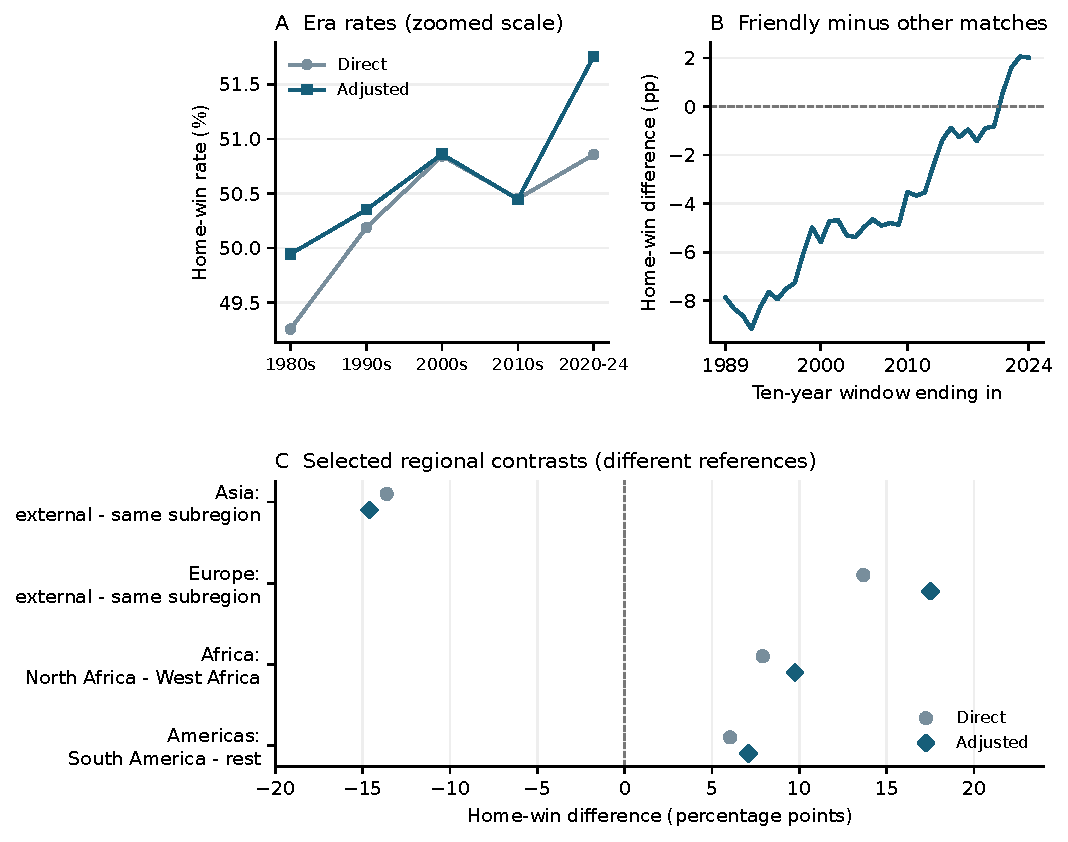
\includegraphics[width=\linewidth]{fig_historical_overview.pdf}
\papercaption{Historical patterns in the common 24,917-match cohort.}{(A) Direct and common-tournament-composition era rates; the vertical axis is truncated and the final era spans five years. (B) Direct friendly-minus-other gaps in 36 overlapping ten-year windows, indexed by ending year. (C) Four predefined regional contrasts: external opponents are outside the home continent; rest denotes other American subregions. Raw and adjusted contrasts use their specified references and do not constitute a regional ranking. The panels present descriptive estimates; uncertainty ranges are reported separately. Complete windows, 29 contrasts, and 155 directional matchups are indexed in the supporting-results guide.}
\label{fig:historical-overview}
\end{figure}

\begin{table}[htbp]
\centering\small
\papercaption{Selected contrasts in the 24,917-match historical sample, in percentage points.}{Ranges are model-conditional envelopes, not unconditional confidence intervals. Each adjustment uses its specified reference; the rows estimate different contrasts.}
\label{tab:historical-contrasts}
\begin{tabular}{p{7.4cm}rr}
\toprule
Contrast and adjustment & Estimate & Conditional range \\
\midrule
2010s minus 1980s, tournament composition & $+0.5019$ & $[-61.66,62.66]$ \\
2020--2024 minus 1980s, tournament composition & $+1.8100$ & $[-100,100]$ \\
Friendly minus other, direct & $-3.2463$ & --- \\
Friendly minus other, era composition & $-2.8831$ & $[-7.2039,1.4377]$ \\
\bottomrule
\end{tabular}
\end{table}

Regional differences depended on opponent composition. Asian home teams won $13.6160$~pp less often against opponents from outside Asia than against opponents from the same study subregion. These groups contained 1,743 and 1,934 matches; the adjusted difference was $-14.6057$~pp. This directional comparison uses the classifications in Section~\ref{sec:data-design}; it does not rank regional ability.

Of 29 predefined regional contrasts, 24 supported adjustment and five lacked required cells. Six of the 24 conditional ranges lay on one side of zero and 18 crossed it; missing comparisons were retained as unsupported. These contrasts are conditional on the observed schedules and reference distributions. Their interpretation also requires consideration of team strength.

The full regional output also contains 155 directional matchups: 153 have observations and 71 support the complete adjustment. Across the historical analyses, 198 of 292 registered targets received model-conditional ranges, while 94 lacked required cells. The 324 sensitivity scenarios produced 26,704 comparison rows; results for modified targets remain descriptive unless the calibration is repeated for those targets. Complete records are listed in the supporting-results guide.

% !TeX root = ../main.tex
\subsection{Strength Estimation: Development, Estimates, and Evaluation}
\label{sec:strength-development}

The strength model produces a time-indexed distribution of latent ability for each team. Figure~\ref{fig:strength-states} illustrates the output for four teams selected for presentation rather than predictive performance. Each point is a pre-match estimate that excludes the selected match's result and incorporates earlier home and away appearances. The means summarize estimated strength, while the whiskers show marginal uncertainty on the fixed performance-noise scale. These marginal summaries distinguish estimated ability from its uncertainty. The joint model uses the strength-difference mixture in Equation~\ref{eq:difference-mixture}, rather than only the displayed mean and standard deviation.

\begin{figure}[htbp]
\centering
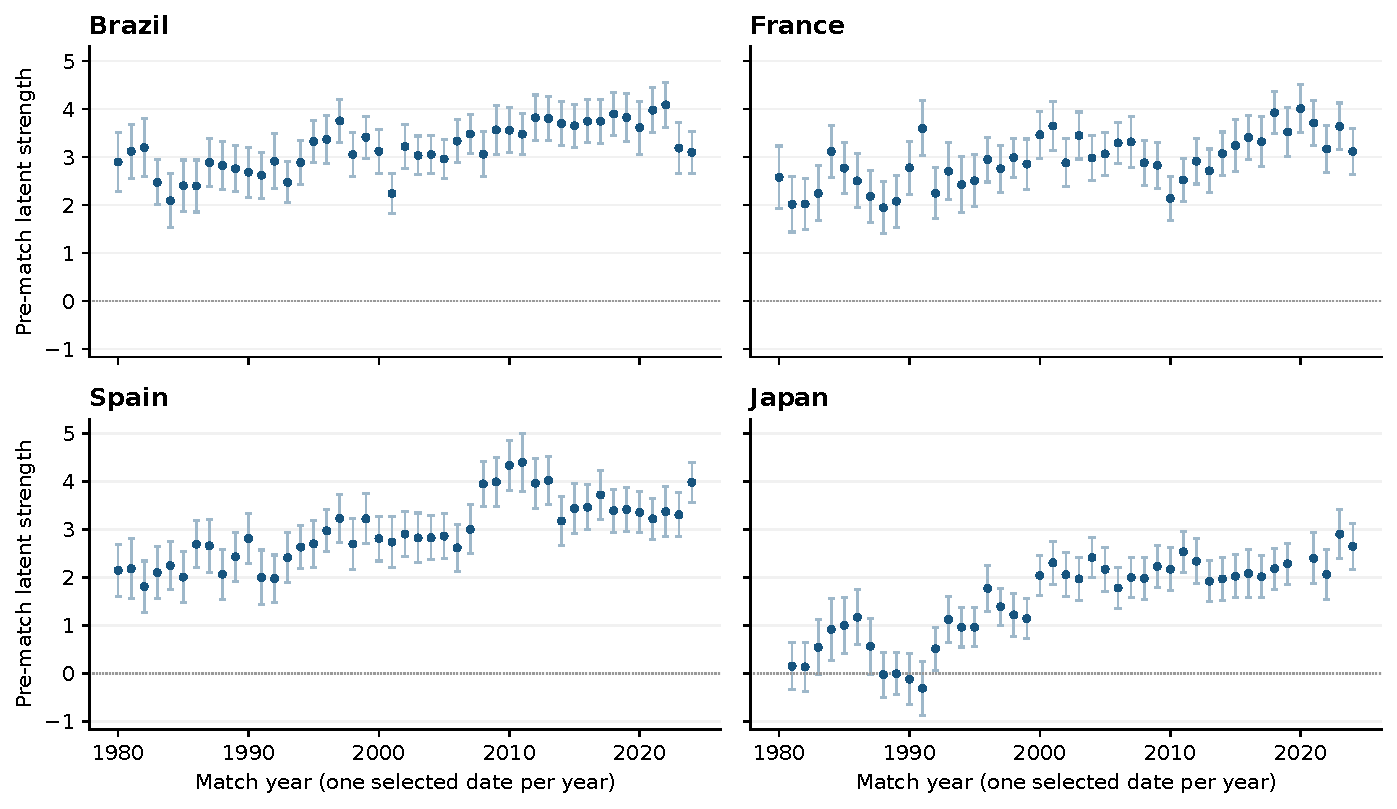
\includegraphics[width=\linewidth]{fig_strength_states.pdf}
\papercaption{Illustrative pre-match strength states, 1980--2024.}{For Brazil, France, Spain, and Japan, each point corresponds to the latest eligible comparative-cohort match in a year, considering both home and away appearances. Whiskers show the marginal mean plus or minus one standard deviation, including jump variance; they do not represent normal-quantile intervals or a world ranking. The zero line is the prior reference. Selected dates do not display every update, and gaps contain no interpolated state estimates.}
\label{fig:strength-states}
\end{figure}

\subsubsection{Model Revisions Informed by Development Results}

Development results informed revisions to the implementation and probability model. They do not establish the optimality of the final rating algorithm. First, explicit expansion of global jump combinations caused excessive memory use. A later moment-collapse approximation still differed from independent numerical references by about $1.328$~pp in match probability, above the original $1$~pp accuracy tolerance. The adopted implementation instead integrates local Poisson counts before processing results, shares a jump variable across a team's same-day matches, and retains the joint covariance. The maximum full-pipeline probability difference between the final ordinary and strict numerical settings was approximately $4.777\times10^{-7}$. This comparison assesses numerical stability for the recorded calculation, rather than the empirical validity of the latent process.

Second, improvements in overall probability scores did not eliminate bias in a particular friendly-match period. Earlier correction candidates underpredicted home wins in the 415 friendlies of 2020--2022 by approximately $3.32$--$4.51$~pp. Separate context fits, switching mixtures, and more flexible matrix corrections did not consistently satisfy the unchanged criteria. Diagnostics indicated distinct errors in probability shape and recent systematic offsets. The final pipeline therefore applies past-only shape correction followed by online residual correction, as described in Section~\ref{sec:strength-method}. For those 415 matches, underprediction decreased to $2.3913$~pp; the corresponding non-friendly bias was $-0.7689$~pp. For 2023--2024, friendly and other-match biases were $+0.9619$ and $+0.3622$~pp. These residual diagnostics do not estimate causal effects of tournament type.

The final comparison included eight candidates, combining two shape mappings with four residual-diffusion values. Two satisfied all prespecified criteria. With diffusion $0.02$, the shared-temperature version had a comparative-cohort loss of $0.890949$, compared with $0.891258$ for the matrix version. These aggregates cover the same 24,917 study matches, not the larger learning population. Candidates were first screened against the criteria, then compared by loss and structural simplicity. The shared-temperature version was selected. The historical data had already been used during development, so these scores do not constitute evaluation on an untouched final holdout. Failed candidates remain documented. The corrections improve the auxiliary probability branch; they do not retrospectively change the strength distributions delivered to the joint analysis.

\subsubsection{Three-Class Evaluation and Remaining Limitations}

Table~\ref{tab:rating-validation} reports the adopted rating-and-correction pipeline on four disjoint historical periods of the comparative cohort. Its target is home win, draw, or away win. The frequency baseline uses earlier venue-specific outcome counts; the internal fixed-step baseline updates both teams from expected-score errors and uses a Davidson-form draw probability. Its registered settings are update size $40$, home offset $100$, and draw parameter $0.75$, on its own rating scale. This internal comparator uses Elo-style updates and is distinct from the official FIFA system. All three issue probabilities before learning the current date's results.

\begin{table}[htbp]
\centering\small
\papercaption{Three-class performance of the final rating pipeline on the comparative cohort.}{The four periods partition 24,917 matches. Loss is three-class negative log probability of the actual result; accuracy selects the most probable of the three outcomes. Bias is predicted minus observed home-win frequency in pp. These results include the probability corrections and reuse development history. They are not directly comparable with the binary scores in Table~\ref{tab:predictive-models}.}
\label{tab:rating-validation}
\begin{tabular*}{\linewidth}{@{\extracolsep{\fill}}lrrrrrr@{}}
\toprule
Period & $n$ & Frequency & Fixed-step & Adopted & Accuracy (\%) & Bias (pp) \\
\midrule
1980--1999 & 8,318 & 1.042385 & 0.939775 & 0.917339 & 56.30 & $+0.1807$ \\
2000--2009 & 6,872 & 1.033723 & 0.895936 & 0.880976 & 59.02 & $-0.0173$ \\
2010--2019 & 6,632 & 1.035877 & 0.880793 & 0.878495 & 60.00 & $+0.0047$ \\
2020--2024 & 3,095 & 1.032750 & 0.863959 & 0.868851 & 60.26 & $-0.3910$ \\
\bottomrule
\end{tabular*}

\end{table}

The pipeline had lower loss than the frequency comparator in every displayed period and lower loss than the fixed-step comparator in the first three. However, in 2020--2024 its loss is $0.868851$ versus $0.863959$, and its accuracy is $60.26\%$ versus $60.97\%$. The loss difference satisfies the prespecified $0.01$ non-inferiority tolerance, although the selected pipeline did not outperform the baseline in every period. The requirements also checked loss improvement of at least $0.005$ against frequency, accuracy no more than $1$~pp below frequency, absolute home-win bias at most $3$~pp, and probability-bin error at most $10$~pp for bins with at least 200 games. Satisfying these tolerances establishes compliance with the operational criteria, rather than general superiority or calibration in every subgroup.

The validation records include 63 targeted tests, independent integration checks, full-history replay, and checkpoint continuation. Simulation under two alternative jump-parameter settings gave nominal $90\%$ strength-difference range coverage of approximately $95.90\%$ and $92.65\%$. These checks assess implementation consistency, numerical approximation, and performance under specified simulation settings. They do not provide observed true-strength labels for real teams. Initialization checks also found 2,905 study matches with a raw home-probability change exceeding $1$~pp under at least one registered alternative, 359 cold starts, and 80 matches whose prior cumulative opponent graph was disconnected. Some match-level initialization effects were substantially larger than the average. The corresponding flags and uncertainty information are retained because a common rating scale does not imply equally reliable comparisons across teams and regions.

The latent strength distributions provide the input to the joint analysis, with the limitations identified above. Corrected three-class probabilities serve as a separate forecasting diagnostic. The common-sample comparison below evaluates the contribution of strength to the binary home-win target and the additional contribution of context.


\subsection{Strength versus Context}
\label{sec:strength-results}
% E32_M0_nested/M1_strength/M3_nested, E32_CONTEXT_*, E32_ADMISSION.

For RQ2, we evaluated background-only, strength-only, and joint predictors on the same 21,413 matches from 1990--2024, using only information available before each prediction. This is a retrospective chronological comparison: the archive also informed development and selection, as described in Section~\ref{sec:data-design}.

Including strength produced the larger reduction in loss (Table~\ref{tab:predictive-models}; Figure~\ref{fig:predictive-models}). Mean log loss declined from $0.671936$ for background alone to $0.566020$ for strength alone and $0.563630$ for the joint predictor. The joint model's relative reductions were $16.12\%$ against background alone and $0.42\%$ against strength alone. The absolute reductions were 0.105916 from background to strength and 0.002390 from strength to the joint model. These are aggregate loss comparisons, not an additive decomposition of information or evidence for individual subgroups. Binary accuracy followed the same ordering: $58.19\%$, $69.83\%$, and $70.01\%$. Accuracy refers to home-win/non-home-win classification and is distinct from relative loss reduction.

\begin{table}[htbp]
\centering\small
\papercaption{Same-match retrospective comparison, 1990--2024 ($n=21,413$).}{Bias is mean predicted home-win probability minus the observed rate, in percentage points. Lower loss and Brier score are preferable.}
\label{tab:predictive-models}
\begin{tabular}{lrrrr}
\toprule
Predictor & Log loss & Brier score & Accuracy (\%) & Bias (pp) \\
\midrule
Background only & 0.671936 & 0.239580 & 58.19 & $-0.0973$ \\
Strength only & 0.566020 & 0.193698 & 69.83 & $+0.9308$ \\
Strength and context & 0.563630 & 0.192657 & 70.01 & $+0.2398$ \\
\bottomrule
\end{tabular}
\end{table}

Adding context also reduced the Brier score from $0.193698$ to $0.192657$ and mean bias from $+0.9308$ to $+0.2398$~pp. The background-only model had the smallest absolute mean bias but the highest loss and Brier score. Agreement with the overall frequency therefore does not establish match-level predictive quality or calibration across probability levels and groups.

\begin{figure}[htbp]
\centering
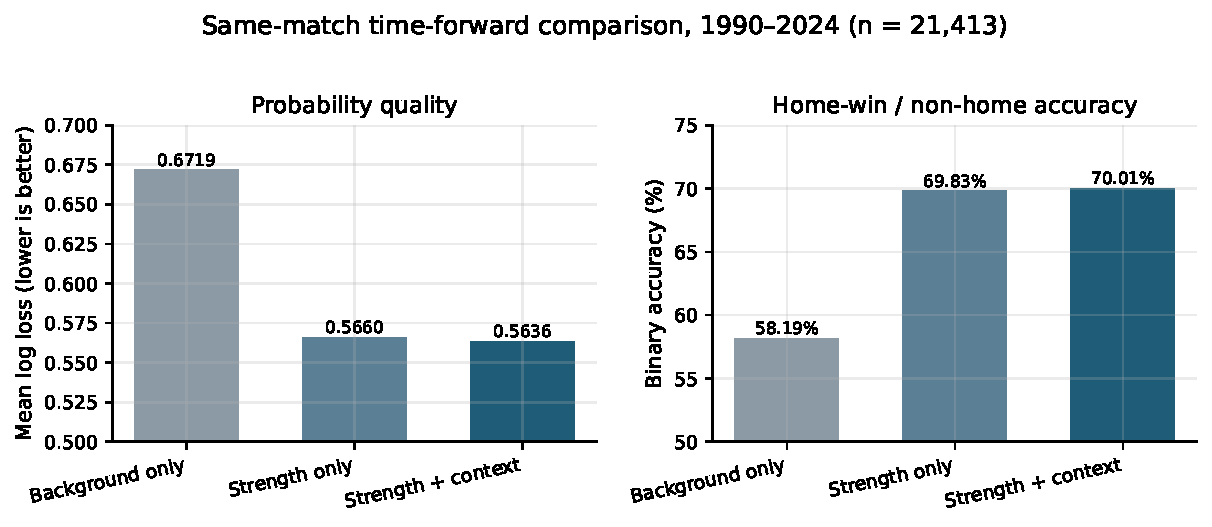
\includegraphics[width=\linewidth]{fig3_model_comparison.pdf}
\papercaption{Strength accounts for most of the improvement in the same-match historical comparison ($n=21,413$, 1990--2024).}{Adding context yields a smaller reduction in loss. Both vertical axes are truncated; magnitudes should be read from the labelled values rather than bar-height ratios. Accuracy is binary; no dependence-adjusted interval from real match data is available for the loss difference.}
\label{fig:predictive-models}
\end{figure}

The separate conditional analysis uses 24,917 matches and a fixed reference. Its strength-adjusted friendly-minus-other contrast was $-3.4957$~pp, with a range from $-7.6712$ to $0.6797$~pp. The paired change after adding strength was $+0.3624$~pp, ranging from $-2.8619$ to $3.5868$~pp. The estimated change was small, and its conditional range did not resolve its direction. Because the reference and target differ, these values cannot be subtracted from the descriptive contrast in Table~\ref{tab:historical-contrasts}.

Of 54 principal quantities assessed by simulation, 30 met the acceptance criteria. For 24 regional changes before and after strength adjustment, the simulated reference values were insufficiently precise for interval validation. These changes remain descriptive; failure to meet the validation criterion does not imply an absence of regional differences. The selected complete-history procedure evaluates conditional comparisons under the specified generators (Section~\ref{sec:evaluation-method}). The separate $0.42\%$ predictive loss gain has no dependence-adjusted interval from real match data, so its persistence in future matches is unresolved.

\subsection{Historical Information and Computational Trade-offs}
\label{sec:history-results}
% E33_LOSS_*, E33_COST_*, E33_SIX_COMBINATIONS, E33_ADAPTIVE.

For RQ3, the historical window used for strength reconstruction was varied separately from the window used to estimate outcome probabilities. Evaluation covered 16,599 matches in 2000--2024, with 9,727 in the main 2010--2024 comparison. Among six tested combinations, cumulative history at both stages gave the lowest main-comparison log loss, $0.559135$ (Figure~\ref{fig:history-windows}). Annual selection using past performance gave $0.560159$. Cumulative history was therefore retained among the tested choices. Earlier matches need not have equal influence on current estimates because the dynamic strength process allows ability to change.

A 12-year outcome-learning window, with cumulative strength estimation fixed, increased loss from $0.559135$ to $0.561131$, or $0.3571\%$ using unrounded values. In the controlled timing batch, this component took $105.29$ rather than $312.58$ seconds, a $66.31\%$ saving. The saving applies to this outcome-fitting component. Other timings in Figure~\ref{fig:history-windows} were obtained in different execution batches and are not standardized benchmarks of the complete pipeline.

\begin{figure}[htbp]
\centering
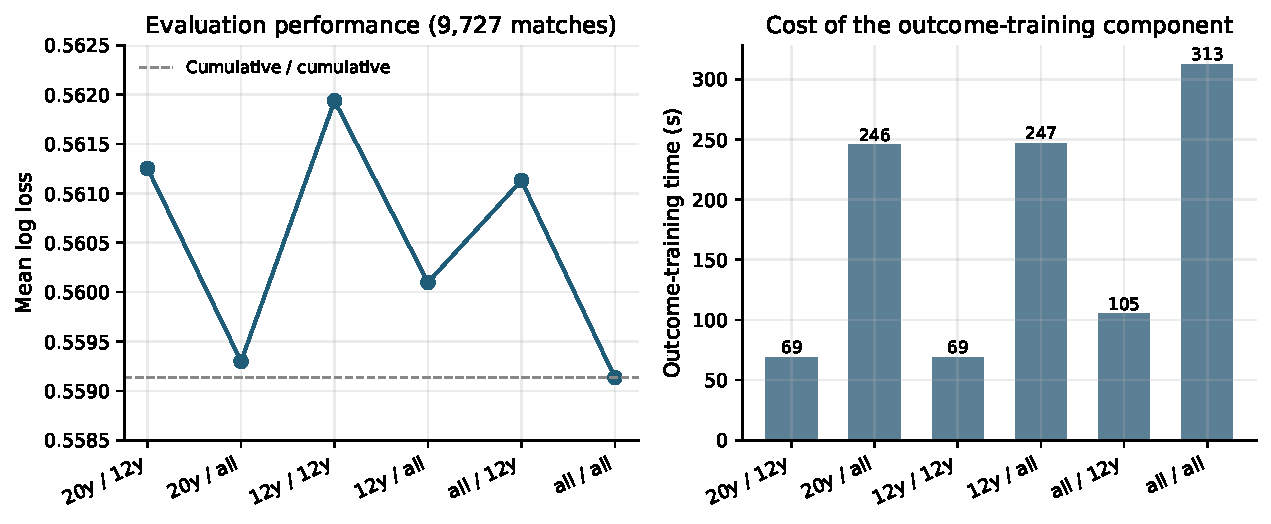
\includegraphics[width=\linewidth]{fig4_history_windows.pdf}
\papercaption{Six tested combinations of rating memory and outcome-learning history.}{Left: loss on the common 2010--2024 sample ($n=9,727$); lines connect discrete candidates for visual reference only. Right: recorded outcome-learning component times, not total pipeline times. The controlled saving in the text compares only all/12y with all/all; timings from other execution batches are not standardized.}
\label{fig:history-windows}
\end{figure}

\subsection{Regional Applicability and Probability Bias}
\label{sec:regional-results}
% E34_*; calibration and composition evidence extended in R20261106-05.

Regional applicability of the joint predictor was assessed using the same 9,727-match main sample. Overall, its log loss was $0.559135$, compared with $0.562000$ for strength alone. This later-period comparison is separate from the 21,413-match evaluation above. Regional scores and bias varied (Table~\ref{tab:regional-diagnostics}; Figure~\ref{fig:regional-metrics}), alongside differences in opponent composition and strength uncertainty. These scores describe performance on the observed matches and do not measure the intrinsic difficulty or quality of a region.

\begin{table}[htbp]
\centering\small
\papercaption{Regional diagnostics, 2010--2024.}{Losses compare identical matches within each row; bias concerns the joint predictor, in percentage points. Interpretations summarize the specified sensitivity checks and do not constitute confidence statements or regional rankings. Americas includes South America; Overall is not an independent additional sample.}
\label{tab:regional-diagnostics}
\begin{tabular}{lrrrrp{3.4cm}}
\toprule
Home region & $n$ & Strength loss & Joint loss & Bias (pp) & Interpretation \\
\midrule
Europe & 3,322 & 0.543239 & 0.539498 & $+0.2189$ & Increment retained \\
Asia & 2,540 & 0.546894 & 0.545041 & $-0.8765$ & Increment retained \\
Africa & 2,058 & 0.613617 & 0.612607 & $+0.6854$ & Increment sensitive \\
Americas & 1,659 & 0.559276 & 0.554578 & $+0.1858$ & Increment retained \\
Oceania & 148 & 0.555130 & 0.549289 & $+2.9572$ & Sparse support \\
Overall & 9,727 & 0.562000 & 0.559135 & $+0.0676$ & Pooled comparison \\
\bottomrule
\end{tabular}
\end{table}

The small loss reductions from adding context in Europe, Asia, and the Americas retained their direction under the specified year/team deletions and alternative reference distributions. These checks provide limited historical support for the additional predictive value of context in these regions. The African increment was more sensitive: its sign reversed after removing 2011 or evaluation matches involving Egypt. This sensitivity concerns the incremental value of context, rather than the predictive value of strength itself in Africa.

The African results also show that a small overall bias can coexist with errors within probability groups. In the low strength-uncertainty category, the 20--40\% predicted-probability bin contained 225 matches, with mean predicted probability $31.21\%$ and observed home-win rate $34.22\%$. In the 60--80\% bin, 287 matches had mean predicted probability $69.17\%$ and observed rate $65.85\%$. The lower bin was underpredicted and the higher bin overpredicted; these directions persisted in the specified checks. Standardizing the broad strength-gap and uncertainty composition narrowed the Africa--Europe loss gap but did not remove it. The remaining discrepancy warrants further investigation, but these comparisons do not identify its cause or demonstrate that uncertainty is fully represented.

South America's ordering relative to the rest of the Americas changed under some deletions and alternative reference distributions. In Oceania, 148 matches were spread over nine adjustment cells, one containing only two matches; deleting matches involving certain teams left a required cell empty. The adjusted comparison was consequently sensitive to a few observations and could become unsupported. These checks held predictions fixed: they did not erase deleted matches from the original learning history or refit each model. They assess the sensitivity of evaluation summaries with predictions held fixed, rather than the performance of a retrained system, and do not yield real-world confidence intervals.

\begin{figure}[htbp]
\centering
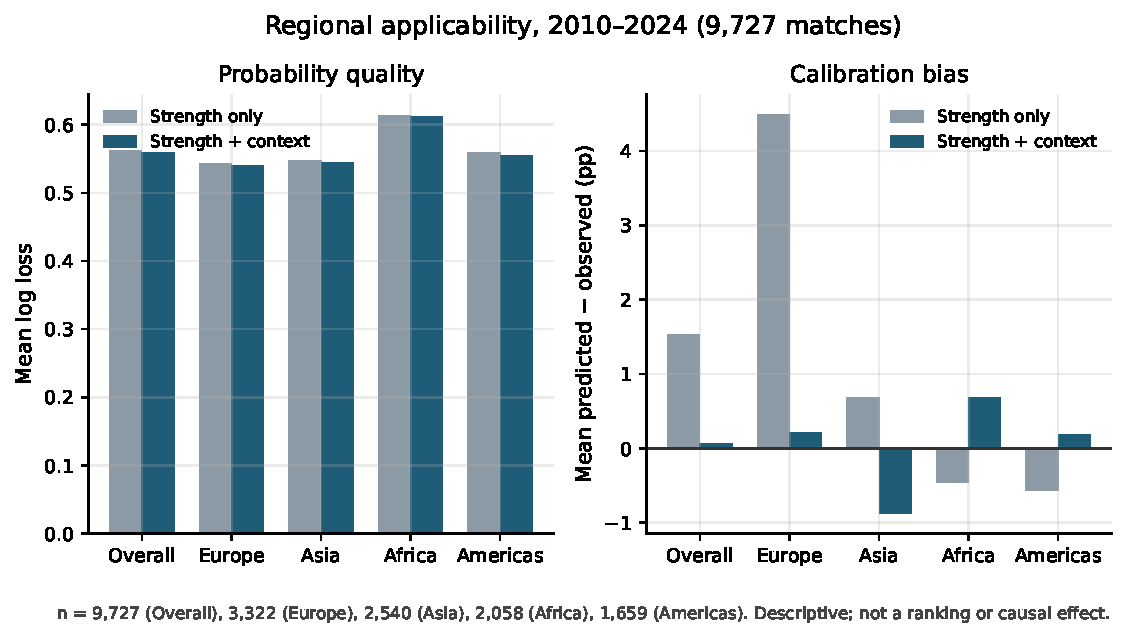
\includegraphics[width=\linewidth]{fig5_regional_metrics.pdf}
\papercaption{Regional probability quality and mean bias on the main 2010--2024 sample.}{The displayed regional groups contain 9,579 of 9,727 matches; Overall additionally includes Oceania's 148 matches. Positive bias means average overprediction. The sensitivity checks discussed in the text supplement these point scores; the scores alone do not establish stable improvements.}
\label{fig:regional-metrics}
\end{figure}

\subsection{Prospective Application}
\label{sec:prospective-results}
% E35_ISSUED and E35_CASE_005/010/048/CZE_SPA.

We applied the model to 52 Nations League fixtures scheduled for 12--17 November 2026 and archived the release on 2 November at 04:07:15 UTC. Dates and pairings were taken from UEFA's schedule~\cite{uefa2026fixtures} and frozen in the issued fixture ledger. Strength estimates used accepted results through 6 October 2026; outcome-model coefficient estimation used data through 29 December 2025. Predictions for both rounds use the same information set. The joint model issued 49 binary predictions and withheld three involving third-country venues outside its application rule. The rating model separately supplied auxiliary win--draw--loss probabilities for all 52 targets; these auxiliary outputs do not replace the withheld joint predictions. The auxiliary three-class outputs are outside the binary model comparison and have not received prospective validation in this release.

Of the 49 joint predictions, 21 favoured a home win and 28 a non-home win; 32 strength-induced ranges crossed the $50\%$ decision threshold. England--Croatia had home-win probability $63.50\%$ (range $43.54$--$81.28\%$); Netherlands--Greece had $50.38\%$ ($31.02$--$69.68\%$); and Czech Republic--Spain had $3.83\%$ ($0.76$--$9.38\%$). For Ukraine--Georgia, the joint estimate was withheld and auxiliary home/draw/away probabilities were $52.26\%$, $25.39\%$, and $22.35\%$. Figure~\ref{fig:issued-forecasts} displays central 90\% ranges from latent strength uncertainty with coefficients fixed; they exclude parameter and model error.

\begin{figure}[htbp]
\centering
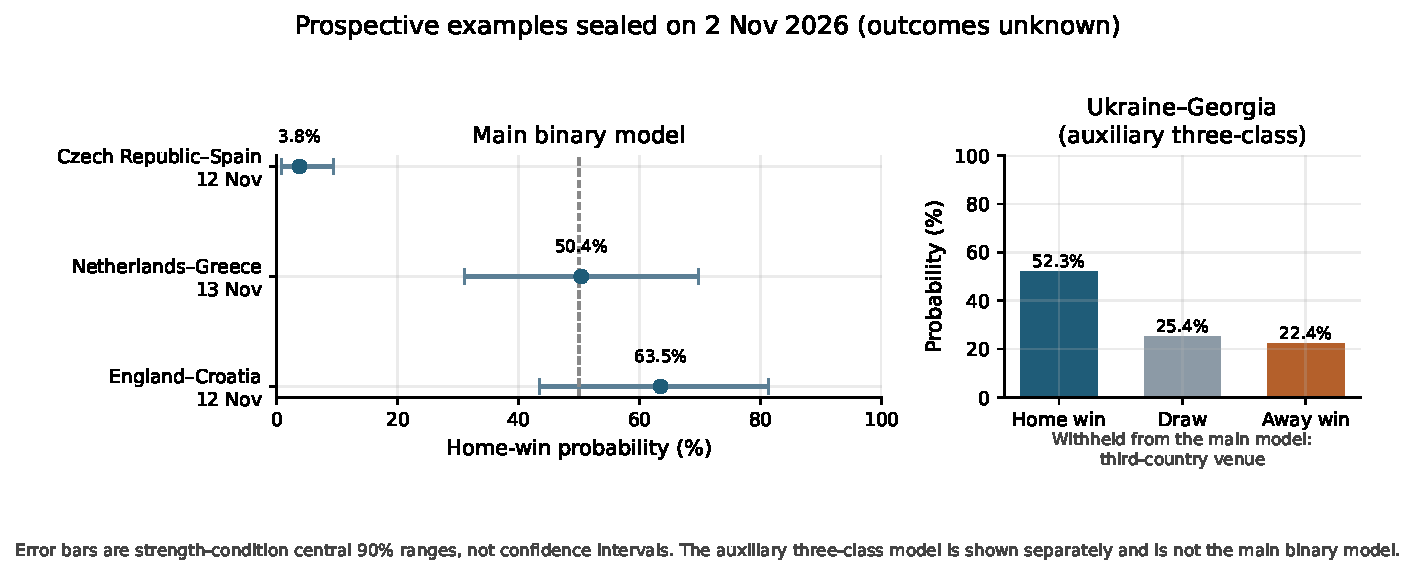
\includegraphics[width=\linewidth]{fig6_forecast_examples.pdf}
\papercaption{Examples from the sealed 2 November 2026 release for 12--17 November fixtures.}{Left: joint binary probabilities with fixed-coefficient latent-strength central 90\% ranges. Right: auxiliary native win--draw--loss probabilities for Ukraine--Georgia, for which the main model withheld its estimate under the venue rule. Actual outcomes are absent; Table~\ref{tab:predictive-models}'s historical accuracy is not an accuracy estimate for these fixtures.}
\label{fig:issued-forecasts}
\end{figure}

The release documents prospective application, with outcomes excluded from the archived ledger. Predictive performance on these fixtures remains unevaluated.

% Final placement is checked in the rendered PDF; no forced float-only page.
